\chapter{Ecuaciones de un péndulo y mov. armónico simple}
\noindent
Estaremos interesados en resolver la ecuación de un péndulo:
\begin{figure}[H]
    \centering
    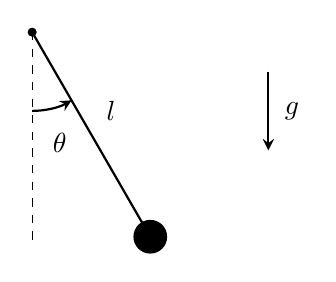
\begin{tikzpicture}
        % Parámetros
        \def\L{3}        % Longitud del péndulo
        \def\LL{2.7}     % Longitud de la vertical
        \def\ang{30}     % Ángulo del péndulo (en grados)

        % Dibujar la línea discontinua vertical
        \draw[dashed] (0,0) -- (0,-\LL);

        % Dibujar el péndulo
        \draw[thick] (0,0) -- ({\L*sin(\ang)}, {-\L*cos(\ang)});

        % Dibujar el círculo al final del péndulo
        \filldraw[thick] ({\L*sin(\ang)}, {-\L*cos(\ang)}) circle (0.2);

        % Indicar el ángulo
        \draw[thick, -stealth] (0,-1) arc[start angle=270, end angle=300, radius=1];
        \node at (0.35, -1.4) {$\theta$};
        \node at (1, -1) {$l$};
        \node at (3.3, -1) {$g$};

        % Flecha hacia abajo para la gravedad
        \draw[thick, -stealth] (3, -0.5) -- (3, -1.5);

        % Dibujar el punto de suspensión
        \filldraw (0,0) circle (0.05);
    \end{tikzpicture}
\end{figure}
\noindent
Pensamos de forma intuitiva que el movimiento de un péndulo se parece al de un muelle si proyectamos sobre el eje $x$ la posición del objeto:
\begin{figure}[H]
    \centering
 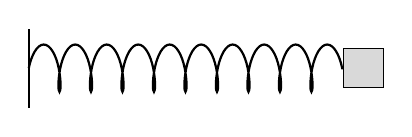
\begin{tikzpicture}
    % Dibuja la pared
    \draw[thick] (0,0.5) -- (0,1.5);

    % Dibuja el muelle
    \draw[thick, decoration={aspect=0.3, segment length=4mm, amplitude=3mm, coil}, decorate] (0,1) -- (4,1);

    % Dibuja el corcho como un cuadrado
    \draw[fill=gray!30] (4,0.75) rectangle (4.5,1.25);
\end{tikzpicture}               
\caption{Muelle atado a la pared.}
\label{fig:muelle}
\end{figure}
\noindent
Tenemos la ecuación del péndulo:
\begin{equation*}
    \ddot{\theta} + \frac{g}{l}\sen\theta = 0
\end{equation*}
Y pensamos que podemos simplificar el estudio de un péndulo al estudio de un muelle con parámetros similares:
\begin{equation*}
    \ddot{\theta} + \frac{g}{l}\theta = 0
\end{equation*}
Y vemos que podemos pensar en que ambas son similares, ya que para $\theta <<1$ tenemos que $\sen\theta\approx \theta$. Esta lección va a versar sobre comparar ecuaciones diferenciales, y tratar de responder a si dos ecuaciones se parecen entonces han de parecerse sus soluciones.

De manera similar, si tienemos una ecuación diferencial con dos condiciones iniciales cercanas, sus soluciones estarán cerca al inicio, pero globalmente pueden tener puntos muy alejados en un mismo tiempo.

\noindent
Formalmente, tendremos dos ecuaciones diferenciales:
\begin{gather*}
    \dot{x} = X(t,x), \qquad x(t_0) = x_0 \\
    \dot{y} = Y(t,y), \qquad y(\tilde{t_0}) = \tilde{x_0}
\end{gather*}
Donde los campos $X$ e $Y$ serán similares y las condiciones iniciales $(t_0,x_0)$ y $(\tilde{t_0},\tilde{x_0})$ serán cercanas.

\section{Dependencia continua respecto a cond. iniciales}
\noindent
En este caso, tendremos una ecuación diferencial
\begin{equation*}
    \dot{x} = X(t,x)
\end{equation*}
dada por un campo $X:D\to \mathbb{R}^d$ continuo para $D\subset \mathbb{R}\times \mathbb{R}^d$ abierto y conexo. Supondremos también unicidad del problema de valores iniciales para toda condición inicial en $D$, ya que si no no tendría sentido plantearse el problema que estamos viendo, porque para un mismo PVI ya podríamos obtener dos soluciones distintas.\\

\noindent
Tomamos ahora dos sucesiones $\{t_{0n}\}\to t_0$ y $\{x_{0n}\}\to x_0$, observamos que como $(t_0,x_0)\in D$ abierto ha de existir $N\in \mathbb{N}$ de forma que $(t_{0n}, x_{0n})\in D$ para todo $n\geq N$.\\

\noindent
Motivados estos pasos, enunciaremos el Teorema que nos interesa en esta sección y que nos interesa demostrar:
\begin{teo}[de la Dependencia Continua]\label{teo:dep_cont}
    Sea $X:D\to \mathbb{R}^d$ un compo continuo con $D\subset \mathbb{R}\times \mathbb{R}^d$ un conjunto abierto y conexo de forma que tenemos unicidad de soluciones para toda condición inicial $(t_0,x_0)\in D$. Dadas dos sucesiones $\{t_{0n}\}\to t_0$ y $\{x_{0n}\}\to x_0$ para cierto punto $(t_0,x_0)\in D$ siendo $x:[a,b]\to \mathbb{R}^d$ solución del PVI
    \begin{equation*}
        \dot{x} = X(t,x), \qquad x(t_0) = x_0
    \end{equation*}
    Entonces:
    \begin{itemize}
        \item $\exists N\in \mathbb{N}$ de manera que si $n\geq N$ entonces podemos encontrar $x_n:[a,b]\to \mathbb{R}^d$ solución del PVI
            \begin{equation*}
                \dot{x} = X(t,x), \qquad x(t_{0n}) = x_{0n}
            \end{equation*}
        \item Además, $\{x_n\}$ converge uniformemente a $x$ en $[a,b]$.
    \end{itemize}
\end{teo}

\begin{ejemplo}
Antes de demostrar este resultado, veamos algunos ejemplos con el fin de aclarar ideas:
\begin{enumerate}
    \item Para cada $n\in \mathbb{N}$ consideramos:
        \begin{equation*}
            \dot{x} = 2x, \qquad x(0) = \frac{1}{n}, \quad n\geq 1
        \end{equation*}
        Tenemos $D=\mathbb{R}\times \mathbb{R}$, hay unicidad de soluciones por ser el campo $C^1$ y las soluciones son:
        \begin{equation*}
            x_n(t) = \frac{1}{n}e^{et}, \quad t\in \mathbb{R}
        \end{equation*}
        Tenemos que:
        \begin{equation*}
            (t_{0n},x_{0n}) = (0, \frac{1}{n}) \to (t_0,x_0) = (0,0)
        \end{equation*}
        El Teorema nos diría que $\{x_n\}\to 0$ uniformemente en cualquier intervalo compacto $[a,b]$ con $0\in [a,b]$, algo que es evidente, puesto que:
        \begin{equation*}
            |x_n(t)| = \frac{1}{n}e^{2t} \leq \frac{1}{n}e^{2b} \qquad \forall t\in [a,b]
        \end{equation*}
        ¿Es importante en el Teorema que el intervalo sea compacto? Si tuviéramos un intervalo no compacto con el extremo derecho no acotado no podríamos realizar la acotación que hemos hecho.

        Al tomar un intervalo no compacto no hay garantías de que se tenga convergencia uniforme.
    \item Podemos considerar ahora para cada $n\geq 1$:
        \begin{equation}\label{eq:sol2}
            \dot{x} = x^2, \qquad x(0) = 1+\frac{1}{n}
        \end{equation}
        Tenemos que la solución para la condición inicial $x(0)=1$ es:
        \begin{equation*}
            x(t) = \frac{1}{1-t}, \quad t\in \left]-\infty,1\right[
        \end{equation*}
        Las soluciones de cada ecuación~\eqref{eq:sol2} los obtenemos por variables separadas:
        \begin{equation*}
            x_n(t) = \frac{-\left(1+\frac{1}{n}\right)}{\left(1+\frac{1}{n}\right)t-1}, \qquad t\in \left]-\infty,\frac{1}{1+\frac{1}{n}}\right[
        \end{equation*}
        Vemos aquí que cada una de las funciones $x_n$ no podrán estar definidas en el mismo sitio que $x$.
\end{enumerate}
\end{ejemplo}

\noindent
El siguiente Lema será de gran utilidad a lo largo de esta sección:
\begin{lema}\label{lema:Ascoli}
    Tenemos una sucesión de funciones $f_n:[a,b]\to \mathbb{R}^d$ de manera que:
    \begin{enumerate}
        \item $\{f_n\}$ es uniformemente acotada y equicontinua.
        \item Existe $f:[a,b]\to \mathbb{R}^d$ de manera que para cada parcial $\{f_{\sigma(n)}\}$ que converge uniformemente se tiene que $f_{\sigma(n)}\to f$ uniformemente.
    \end{enumerate}
    Entonces $\{f_n\}\to f$ convergente uniformemente en $[a,b]$.
    \begin{proof}
         % // TODO: Probar
    \end{proof}
\end{lema}

\noindent
La demostración del Lema anterior es similar al enunciado:
\begin{center}
    Sea $X$ un espacio métrico y $\{x_n\}$ una sucesión en $X$ de manera que existe un compacto $K\subset X$ que contiene a la sucesión y $\exists x\in X$ de forma que para toda parcial convergente $\{x_{\sigma(n)}\}$ se tiene que $\{x_{\sigma(n)}\}\to x$.

    Entonces $\{x_n\}\to x$.
\end{center}
De hecho, la demostración del Lema puede hacerse como un caso particular de este enunciado.

\subsection{Demostración del Teorema de la Dependencia Continua}
\noindent
Realizaremos una estrategia similar a la que hicimos para el de Cauchy-Peano, pasándonos a un caso con un dominio más fácil y en el que el campo esté acotado. Así, la demostración tendrá dos pasos:
\begin{description}
    \item [Paso 1.] Supondremos que $D=\mathbb{R}\times \mathbb{R}^d$ y que existe $M\geq 0$ de forma que:
        \begin{equation*}
            \|X(t,x)\|\leq M \qquad \forall (t,x)\in D
        \end{equation*}
        Estas hipótesis nos quita la primera parte\footnote{La parte de que existe $N\in \mathbb{N}$ de manera que las sucesiones también estén definidas en el mismo intervalo, pues cualquier solución de este PVI estará definida en todo $\mathbb{R}$ por el Teorema de crecimiento lineal.} Solo supondremos unicidad para $(t_0,x_0)$.
    \item [Paso 2.] Tomamos el caso general y lo pasaremos a un caso que se reduce al del paso anterior.
\end{description}

\subsubsection{Demostración del Paso 1}
% // TODO: COpiar aquí el enunciado que se va a probar, una vez entienda la demostración
\noindent
Sea $x_n(t)$ la solución al PVI:
\begin{equation*}
    \dot{x} = X(t,x), \qquad x(t_{0n}) = x_{0n}
\end{equation*}
Sabemos por el Teorema de crecimiento lineal (Teorema~\ref{teo:crecimiento_lineal}) que $x_n(t)$ está definida en todo $\mathbb{R}$. Como $\{t_{0n}\}\to t_0$, existirá $N\in \mathbb{N}$ de manera que para $n\geq N$ tendremos que $a<t_{0n}<b$.\\

\noindent
Si tomamos $f_n = x_n\big|_{[a,b]}$, buscamos aplicar el Lema~\ref{lema:Ascoli}, por lo que lo primero es buscar demostrar que $f_n$ es uniformemente acotada y equicontinua, algo que nos es ya fácil, puesto que:
\begin{equation*}
    \dot{x}_n(t) = X(t,x_n(t)) \quad\Longrightarrow\quad \|\dot{x}_n(t)\| = \|X(t,x_n(t))\| \leq M \quad \forall t\in [a,b]
\end{equation*}
Así, tenemos en un primer lugar que:
\begin{equation*}
    \|x_n(t) - x_n(s)\| \leq M|t-s| \qquad \forall t,s\in [a,b]
\end{equation*}
Donde hemos aplicado la desigualdad (vectorial) del Valor Medio, obteniendo la equicontinuidad de $\{x_n\}$. Ahora, para la acotación uniforme, tenemos que:
\begin{align*}
    \|x_n(t)\| \leq \|x_n(t) - x_n(t_{0n})\| + \|x_n(t_{0n})\| &\leq M|t-t_{0n}| + \|x_{0n}\| \\
                                                               &\leq M(b-a) + C
\end{align*}
Donde usamos que $\{\|x_{0n}\|\}$ es una sucesión convergente, por lo que podemos acotarla por una determinada constante $C\in \mathbb{R}$. Nos falta comprobar que ``tiene un único punto de acumulación''.\\

\noindent
Para elo, sea $\{x_{\sigma(n)}\}$ una parcial de $\{x_n\}$ convergente uniformemente en $[a,b]$ a cierta función $x^\ast$, usando que cada $x_{\sigma(n)}$ es solución del PVI\footnote{Como vamos a pasar al límite es mejor trabajar con integrales que con derivadas.}:
\begin{equation*}
    x_{\sigma(n)}(t) = x_{0\sigma(n)} + \int_{t_{0\sigma(n)}}^{t} X(s,x_{\sigma(n)}(s))~ds 
\end{equation*}
Partiendo la integral en dos:
\begin{equation}\label{eq:igualdad_int}
    x_{\sigma(n)}(t) = x_{0\sigma(n)} + \int_{t_{0\sigma(n)}}^{t_0} X(s,x_{\sigma(n)}(s))~ds  + \int_{t_0}^{t} X(s,x_{\sigma(n)}(s))~ds 
\end{equation}
Donde podemos acotar la primera integral, pues el campo $X$ está acotado por $M$ y tendremos que la primera integral tendrá a $0$, pues $\{t_{0\sigma(n)}\}\to t_0$:
\begin{equation*}
    \int_{t_{0\sigma(n)}}^{t_0} X(s,x_{\sigma(n)}(s))~dts \leq M|t_0 - t_{0\sigma(n)}| \to 0
\end{equation*}
Ahora, para la segunda integral:
\begin{equation*}
    \int_{t_0}^{t} X(s,x_{\sigma(n)}(s))~ds  \to \int_{t_0}^{t} X(s,x^\ast(s))~ds 
\end{equation*}
Donde hemos aplicado el Teorema de la convergencia dominada, pues para cada $s$ tenemos que la función $s\mapsto X(s,x_{\sigma(n)}(s))$ está acotada por $M$. Pasando al límite en la igualdad~\ref{eq:igualdad_int}:
\begin{equation*}
    x^{\ast}(t) = x_0 + \int_{t_0}^{t} X(s,x^{\ast}(s))~ds 
\end{equation*}
Ahora, tenemos que $x^\ast:[a,b]\to \mathbb{R}^d$ es continua y cumple la ecuación integral superior, que es equivalente al problema de valores iniciales. Sin embargo, para la condición inicial $(t_0,x_0)$ estábamos suponiendo que había unicidad de soluciones y $x$ era una solución, por lo que $x=x^\ast$, como queríamos probar. Aplicando el Lema~\ref{lema:Ascoli} acabamos la demostración.\\

\subsubsection{Retracciones}
\noindent
Para tratar el caso general necesitaremos algunas ideas sobre retracciones:

\begin{definicion}
    Necesitamos manejar los conceptos:
    \begin{itemize}
        \item Dada una aplicación $\varphi:[a,b]\to \mathbb{R}^d$ continua y fijado $\rho>0$, consideramos el \textit{tubo} que en cada instante $t\in [a,b]$ tiene centro $\varphi(t)$ y radio $\rho$:
        \begin{equation*}
            T = \{(t,x)\in \mathbb{R} : t\in [a,b], \|x-\varphi(t)\| \leq \rho\}
        \end{equation*}
        \item Una \textit{retracción} es una aplicación $r:\mathbb{R}\times \mathbb{R}^d\to T$ continua de forma que:
            \begin{equation*}
                r\big|_T = id
            \end{equation*}
    \end{itemize}
\end{definicion}

\begin{ejemplo}
    Veamos que podemos ``retraer'' todo $\mathbb{R}\times \mathbb{R}^d$ a un tubo:\\

    \noindent
    Dado un tubo $T$, con ayuda de la aplicación $\sigma:\mathbb{R}\to [a,b]$ dada por:
    \begin{equation*}
        \sigma(t) = \left\{\begin{array}{ll}
                t & \text{si\ } t\in [a,b] \\
            a & \text{si\ } t<a \\
            b &\text{si\ } t>b
        \end{array}\right. 
    \end{equation*}
    Podemos tomar $r_1:\mathbb{R}\times \mathbb{R}^d\to [a,b]\times \mathbb{R}^d$ dada por:
    \begin{equation*}
        r_1(t,x) = (\sigma(t),x)
    \end{equation*}
    Que retrae todo el espacio-tiempo a una banda vertical. Ahora, consideramos también $r_2:[a,b]:\mathbb{R}^d\to T$ dada por:
    \begin{equation*}
        r_2(t,x) = \left\{\begin{array}{ll}
                (t,x) & \text{si\ } (t,x)\in T \\
                \left(t,\varphi(t)+\rho\frac{x-\varphi(t)}{\|x-\varphi(t)\|}\right)& \text{si\ } (t,x)\notin T
        \end{array}\right. 
    \end{equation*}
    Vemos que $r_1$ y $r_2$ son continuas\footnote{Para $r_2$ podemos aplicar el Lema del Pegado.}. Finalmente consideramos $r=r_2\circ r_1:\mathbb{R}\times \mathbb{R}^d\to T$, que es continua y claramente $r\big|_T = id$.
\end{ejemplo}

\subsubsection{Demostración del Paso 2}
\noindent
Recordando el enunciado del Teorema que queremos probar:
\begin{teo}[de la Dependencia Continua] 
    Sea $X:D\to \mathbb{R}^d$ un compo continuo con $D\subset \mathbb{R}\times \mathbb{R}^d$ un conjunto abierto y conexo de forma que tenemos unicidad de soluciones para toda condición inicial $(t_0,x_0)\in D$. Dadas dos sucesiones $\{t_{0n}\}\to t_0$ y $\{x_{0n}\}\to x_0$ para cierto punto $(t_0,x_0)\in D$ siendo $x:[a,b]\to \mathbb{R}^d$ solución del PVI:
    \begin{equation*}
        \dot{x} = X(t,x), \qquad x(t_0) = x_0
    \end{equation*}
    Entonces:
    \begin{itemize}
        \item $\exists N\in \mathbb{N}$ de manera que si $n\geq N$ entonces $x_n:[a,b]\to \mathbb{R}^d$ es solución del PVI:
            \begin{equation*}
                \dot{x} = X(t,x), \qquad x(t_{0n}) = x_{0n}
            \end{equation*}
        \item Además, $\{x_n\}$ converge uniformemente a $x$ en $[a,b]$.
    \end{itemize}
\end{teo}

% // TODO: Enunciar esto bien al inicio de la sección 3.1.1.
\noindent
Hemos ya probado el Teorema para el caso particular $D=\mathbb{R}\times \mathbb{R}^d$ y de forma que existe $M\geq 0$ con:
\begin{equation*}
    \|X(t,x)\| \leq M \qquad \forall (t,x)\in D
\end{equation*}
Suponiendo solo unicidad del PVI para $(t_0,x_0)$.

\begin{proof}
    Observemos que el conjunto:
    \begin{equation*}
        \{(t,x(t)) : t\in [a,b]\} \subset D
    \end{equation*}
    es un conjunto compacto. Por ser $D$ abierto, existe $\rho>0$ de forma que:
    \begin{equation*}
        T = \{(t,x)\in \mathbb{R}\times \mathbb{R}^d : t\in [a,b], \|x-x(t)\| \leq \rho\} \subset D
    \end{equation*}

    \begin{figure}[H]
        \centering
        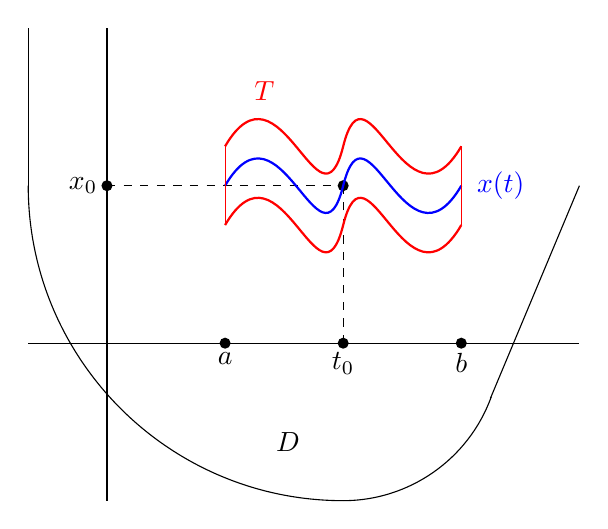
\begin{tikzpicture}
        \draw (-1,0) -- (6,0);
        \draw (0,-2) -- (0,4);
        \fill (0,2) circle(2pt) node[left] {$x_0$};
        \fill (3,0) circle(2pt) node[below] {$t_0$};
        \fill (1.5,0) circle(2pt) node[below] {$a$};
        \fill (4.5,0) circle(2pt) node[below] {$b$};
        \fill (3,2) circle(2pt) node[] {};
        \draw[dashed] (0,2) -- (3,2);
        \draw[dashed] (3,0) -- (3,2);

        \draw (3,2) ++(180:4) arc (180:270:4);
        \draw (-1,2) -- (-1,4);
        \draw (3,0) ++(270:2) arc (270:340:2);
        \draw (4.87,-0.7) -- (6,2);
        \fill (2.3,-1.5) node[above] {$D$};

        \fill[blue] (5,2) node[] {$x(t)$};
        \fill[red] (2,3.2) node[] {$T$};

        % Curva original (~)
        \draw[thick, blue]
            (1.5,2)
            .. controls (2.2,3.2) and (2.7,0.8) ..
            (3,2)
            .. controls (3.3,3.2) and (3.8,0.8) ..
            (4.5,2);

        \begin{scope}[yshift=+0.5cm]
            \draw[thick, red]
                (1.5,2)
                .. controls (2.2,3.2) and (2.7,0.8) ..
                (3,2)
                .. controls (3.3,3.2) and (3.8,0.8) ..
                (4.5,2);
        \end{scope}

        \begin{scope}[yshift=-0.5cm]
            \draw[thick, red]
                (1.5,2)
                .. controls (2.2,3.2) and (2.7,0.8) ..
                (3,2)
                .. controls (3.3,3.2) and (3.8,0.8) ..
                (4.5,2);
        \end{scope}

        \draw[red] (1.5,2.5) -- (1.5,1.5);
        \draw[red] (4.5,2.5) -- (4.5,1.5);
        \end{tikzpicture}
    \end{figure}

    \noindent
    Definimos ahora el campo $\tilde{X}:\mathbb{R}\times \mathbb{R}^d\to \mathbb{R}^d$ dada por (siendo $r:\mathbb{R}\times\mathbb{R}^d\to T$ la retracción vista en el ejemplo anterior):
    \begin{equation*}
        \tilde{X}(t,x) = X(r(t,x))
    \end{equation*}
    Vemos que $\tilde{X}(t,x) = X(t,x)\quad \forall (t,x)\in T$. Como $T$ es compacto, existe $M\geq 0$ de forma que:
    \begin{equation*}
        \|X(t,x)\| \leq M \qquad \forall (t,x)\in T
    \end{equation*}
    Ahora, como $\tilde{X}(\mathbb{R}\times \mathbb{R}^d)= X(T)$, tenemos que:
    \begin{equation*}
        \|\tilde{X}(t,x)\|\leq M \qquad \forall (t,x)\in \mathbb{R}\times \mathbb{R}^d
    \end{equation*}
    Falta ver que hay unicidad para el problema:
    \begin{equation}\label{eq:pvi_mod}
        \dot{x} = \tilde{X}(t,x),\qquad x(t_0) = x_0
    \end{equation}
    Observemos que solo sabemos que hay unicidad para los PVI:
    \begin{equation*}
        \dot{x} = X(t,x),\qquad x(t_1) = x_1
    \end{equation*}
    Para todo $(t_1,x_1)\in D$. Sin embargo, vemos que $x(t)$ es solución de~\eqref{eq:pvi_mod}, ya que:
    \begin{equation*}
        \dot{x}(t) = X(t,x(t)) \AstIg \tilde{X}(t,x(t)) \qquad \forall t\in [a,b]
    \end{equation*}
    Donde en $(\ast)$ hemos usado que $Im x \subset T$, al ser $x(t)$ el eje del tubo.\\

    \noindent
    Sea $\tilde{x}:[a,b]\to \mathbb{R}^d$ solución del PVI~\eqref{eq:pvi_mod}, queremos probar entonces que $\tilde{x}(t) = x(t)\quad \forall t\in [a,b]$. Para ello, si tomamos:
    \begin{equation*}
        \cc{I} = \{t\in [a,b] : x(t) = \tilde{x}(t)\}
    \end{equation*}
    Que es un conjunto no vacío ($t_0\in \cc{I}$), cerrado y falta ver que es abierto relativo a $[a,b]$. Para ello, si $t_\ast \in \cc{I}$, tenemos entonces que $\tilde{x}(t_\ast) = x(t_\ast)$ por ser ambas continuas tenemos que existe $\delta>0$ de forma que:
    \begin{equation*}
        \|x(t) - \tilde{x}(t)\| < \rho \qquad \forall t\in [t_\ast-\delta,t_\ast+\delta]\cap[a,b]
    \end{equation*}
    Así, tenemos que:
    \begin{equation*}
        (t,\tilde{x}(t))\in T \qquad \forall t\in [t_\ast-\delta,t_\ast+\delta]\cap[a,b] = J
    \end{equation*}
    Pero ahora vemos que $\tilde{x}\big|_J$ es solución del PVI (tomando $x_\ast = x(t_\ast)$):
    \begin{equation*}
        \dot{y} = X(t,y), \qquad y(t_\ast) = x_\ast 
    \end{equation*}
    Finalmente, por la unicidad concluimos que $x\big|_J = \tilde{x}\big|_J$.\\

    \noindent
    En definitiva, hemos probado que $\cc{I}= [a,b]$, por lo que tenemos unicidad para el PVI~\eqref{eq:pvi_mod} y podemos aplicar el Paso 1 que ya habíamos probado.\\

    \noindent
    Ahora, para el problema:
    \begin{equation*}
        \dot{x} =\tilde{X}(t,x), \qquad x(t_{0n}) = x_{0n}
    \end{equation*}
    Tomamos una solución $\tilde{x}_n(t)$ definida en $[a,b]$ (el campo $\tilde{X}$ está acotado, por lo que sabemos que podemos prolongarla a todo $[a,b]$) y sabemos ya que $\{\tilde{x}_n\}$ converge uniformemente a $\tilde{x} = x$ en $[a,b]$. Si conseguimos probar que a partir de cierto $N\in \mathbb{N}$ tenemos que $\tilde{x}_n$ son soluciones del PVI:
    \begin{equation*}
        \dot{x} = X(t,x), \qquad x(t_{0n}) = x_{0n}
    \end{equation*}
    Entonces tendremos ya el Teorema de dependencia continua demostrado. Para ello, basta ver que $\exists N\in \mathbb{N}$ de forma que para $n\geq N$ tenemos que:
    \begin{equation*}
        (t,\tilde{x}_n(t)) \in T\qquad \forall t\in [a,b]
    \end{equation*}
    Esta condición nos la da la definición de convergencia uniforme para la sucesión $\{\tilde{x}_n\}$, dado $\rho >0$ tenemos que existe $N\in \mathbb{N}$ de forma que si $n\geq N$ entonces:
    \begin{equation*}
        \|\tilde{x}_n(t) - x(t)\| < \rho \qquad \forall t\in [a,b]
    \end{equation*}
\end{proof}

\section{Ecuaciones diferenciales con parámetros} % // TODO: Reformular esto como teorema
\noindent
Tendremos ahora una ecuación diferencial de la forma:
\begin{equation*}
    \dot{x} = X(t,x,\lm)
\end{equation*}
para $X:D\times \Lambda\to \mathbb{R}^d$ continua donde $D$ es un abierto conexo de $\mathbb{R}^d$ y $\Lambda$ es un abierto conexo de $\mathbb{R}^m$. Por tanto, no tenemos una ecuación diferencial, sino una familia de ecuaciones diferenciales, una para cada $\lm\in \Lambda$. Supondremos que tenemos una condición inicial $(t_0,x_0)\in D$ fija.\\

\noindent
Supondremos además que tenemos unicidad de:
\begin{equation*}
    \left\{\begin{array}{l}
        \dot{x} = X(t,x,\lm) \\
        x(t_\ast) = x_\ast
    \end{array}\right.
\end{equation*}
para todo $\lm\in \Lambda$ y para toda condición inicial $(t_\ast,x_\ast)\in D$. Así, las soluciones del PVI serán funciones $x(t,\lm)$.\\

\noindent
Finalmente, tendremos $\{\lm_n\}\to \lm_\ast$ para $\lm_n,\lm_\ast \in \Lambda$ y de forma que $x(t,\lm_\ast)$ esté definida en $[a,b]$ con $a<t_0<b$. De esta situación podremos deducir que existe $N\in \mathbb{N}$ de forma que $x(t,\lm_n)$ está definida en $[a,b]$ para todo $n\geq N$ y $\{x(t,\lm_n)\}\to x(t,\lm_\ast)$ converge uniformemente en $t\in [a,b]$.

\begin{ejemplo}
    Para cada $n\geq 1$ consideramos la ecuación:
    \begin{equation*}
        \dot{x} = \frac{1}{n}x, \qquad x(0) = 1
    \end{equation*}
    Tenemos que su solución es: 
    \begin{equation*}
        x_n(t) = e^{\frac{1}{n}t}, \qquad t\in \mathbb{R}
    \end{equation*}
    Para este problema tenemos $D = \mathbb{R}^2$, $\Lambda = \mathbb{R}$ y tenemos el campo:
    \begin{equation*}
        X(t,x,\lm) = \lm x
    \end{equation*}
    Vemos que hay unicidad para cualquier condición inicial y tendríamos $\lm_n = \frac{1}{n}$ y $\lm_\ast = 0$. Observamos que $x(t,\lm_\ast) = 1 \quad \forall t\in \mathbb{R}$. Estamos en todas las condiciones del Teorema, salvo que tenemos soluciones que no están definidas en un intervalo compacto. En cada intervalo compacto el Teorema será cierto, pero en todo $\mathbb{R}$ no tendremos convergencia uniforme a la función constantemente igual a 1.
\end{ejemplo}

\noindent
Procedemos ahora con la demostración de este Teorema, que se basa en tratar el parámetro como incógnita:
\begin{proof} % // TODO: Demstración del Teorema
    Sea $z = (x,\lm)$, consideramos el sistema con condiciones iniciales:
    \begin{equation*}
        \left\{\begin{array}{ll}
            \dot{x} = X(t,x,\lm), & x(t_0) = x_0 \\
            \dot{\lm} = 0, & \lm(t_0) = \lm_n 
        \end{array}\right.
    \end{equation*}
    Tenemos ahora un sistema $\dot{z} = Z(t,z)$ con $Z:D\times \Lambda\to \mathbb{R}^{d+m}$ dado por:
    \begin{equation*}
        Z(t,z) = (X(t,x,\lm),0)
    \end{equation*}
    que es continuo y está definido en un conjunto abierto y conexo. Tenemos para cada $n\in \mathbb{N}$ una condición inicial $z(t_0) = z_n = (x_0, \lm_n)$, así como $z_\ast = (x_0,\lm_\ast)$.\\

    \noindent
    Es claro que la unicidad de este problema de valores iniciales depende de las hipótesis fijadas. Si consideramos ahora $z_\ast(t)$ definida en $[a,b]$, podemos aplicar el Teorema~\ref{teo:dep_cont} para obtener la tesis que buscamos.
\end{proof}

\section{Aproximación del péndulo por oscilador armónico}
\noindent
Antes de comenzar la sección, debemos indicar:
\begin{notacion}
    Sean $f$ y $g$ dos funciones, diremos que:
    \begin{equation*}
        f(x) = O(g(x))
    \end{equation*}
    en cierto dominio siempre que $\exists C>0$ de forma que $|f(x)| \leq Cg(x)$ en dicho dominio.\\

    \noindent
    Usaremos también:
    \begin{equation*}
        f(x) = o(g(x)), \quad x\to 0
    \end{equation*}
    si se tiene que:
    \begin{equation*}
        \lim_{x\to0}\frac{f(x)}{g(x)} = 0
    \end{equation*}
\end{notacion}

\begin{ejemplo}
    Vemos que:
    \begin{enumerate}
        \item $x^7 = O(x^6)$ en $[0,1]$.
        \item $x^7 = O(x^6)$ cuando $x\to 0$.
        \item $x^6 = O(x^7)$ cuando $x\to +\infty$.
        \item $x^7 = o(x^6)$ cuando $x\to 0$.
        \item $x^6\sen\left(\frac{1}{x}\right) = O(x^6)$ cuando $x\to 0$ pero $x^6\sen\left(\frac{1}{x}\right) \neq o(x^6)$ cuando $x\to 0$.
    \end{enumerate}
\end{ejemplo}

\noindent
Recordando el problema, tenemos:
\begin{figure}[H]
    \centering
    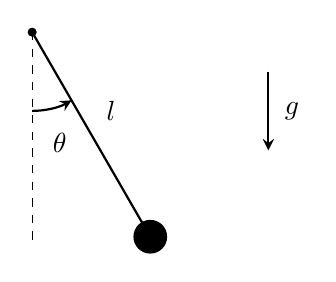
\begin{tikzpicture}
        % Parámetros
        \def\L{3}        % Longitud del péndulo
        \def\LL{2.7}     % Longitud de la vertical
        \def\ang{30}     % Ángulo del péndulo (en grados)

        % Dibujar la línea discontinua vertical
        \draw[dashed] (0,0) -- (0,-\LL);

        % Dibujar el péndulo
        \draw[thick] (0,0) -- ({\L*sin(\ang)}, {-\L*cos(\ang)});

        % Dibujar el círculo al final del péndulo
        \filldraw[thick] ({\L*sin(\ang)}, {-\L*cos(\ang)}) circle (0.2);

        % Indicar el ángulo
        \draw[thick, -stealth] (0,-1) arc[start angle=270, end angle=300, radius=1];
        \node at (0.35, -1.4) {$\theta$};
        \node at (1, -1) {$l$};
        \node at (3.3, -1) {$g$};

        % Flecha hacia abajo para la gravedad
        \draw[thick, -stealth] (3, -0.5) -- (3, -1.5);

        % Dibujar el punto de suspensión
        \filldraw (0,0) circle (0.05);
    \end{tikzpicture}
\end{figure}
Que se rige por la ecuación diferencial:
\noindent
\begin{equation*}
    \ddot{\theta} + \frac{g}{l}\sen \theta = 0
\end{equation*}
Y supondremos que el péndulo no tiene muchas oscilaciones, es decir, lo hemos cogido y lo hemos soltado tras cierto desplazamiento.
\begin{equation*}
    \theta(0) = \varepsilon, \qquad \dot{\theta}(0) = 0
\end{equation*}
Tenemos una solución $\theta(t,\varepsilon)$. Intuitivamente pensamos que la sombra del péndulo se parece al movimiento que hace un muelle:
\begin{figure}[H]
    \centering
 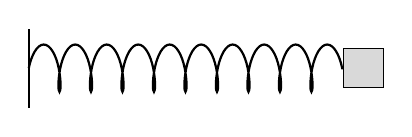
\begin{tikzpicture}
    % Dibuja la pared
    \draw[thick] (0,0.5) -- (0,1.5);

    % Dibuja el muelle
    \draw[thick, decoration={aspect=0.3, segment length=4mm, amplitude=3mm, coil}, decorate] (0,1) -- (4,1);

    % Dibuja el corcho como un cuadrado
    \draw[fill=gray!30] (4,0.75) rectangle (4.5,1.25);
\end{tikzpicture}               
\caption{Muelle atado a la pared.}
\label{fig:muelle}
\end{figure}
\noindent
Así, en este caso queremos resolver:
\begin{equation*}
    \ddot{\theta} + \frac{g}{l}\theta = 0, \qquad \theta(0) = \varepsilon,\quad \dot{\theta}(0) = 0
\end{equation*}
Y a diferencia de la ecuación del péndulo, sabemos que sus soluciones son:
\begin{equation*}
    \theta(t) = \varepsilon\cos\left(\sqrt{\frac{g}{l}}t\right)
\end{equation*}~\\

\noindent
Para formalizar esta idea, dado $T>0$ tenemos el problema:
\begin{equation*}
    \left\{\begin{array}{l}
        \ddot{\theta} + \frac{g}{l}\sen\theta = 0 \\
        \theta(0) = \varepsilon,\quad \dot{\theta}(0) = 0
    \end{array}\right.
\end{equation*}
Y tendremos la solución:
\begin{align*}
    \theta(t,\varepsilon) &= \varepsilon \cos\left(\sqrt{\frac{g}{l}}t\right) + o(\varepsilon) \\
    \dot{\theta}(t,\varepsilon) &= -\varepsilon \sqrt{\frac{g}{l}}\sen\left(\sqrt{\frac{g}{l}}t\right) + o(\varepsilon)
\end{align*}
si $\varepsilon\to 0$ uniformemente\footnote{Es decir, la convergencia no pasa solo en cada instante de tiempo sino en todos a la vez.} en $t\in [-T,T]$.\\

\noindent
Tomaremos para $\varepsilon>0$:
\begin{equation*}
    \left\{\begin{array}{l}
        \theta = \varepsilon y_1 \\
        \dot{\theta} = \varepsilon y_2
    \end{array}\right.
\end{equation*}
Con lo que:
\begin{gather*}
    \varepsilon\dot{y}_1 = \dot{\theta} = \varepsilon y_2 \\
    \varepsilon \dot{y}_2 = \ddot{\theta} = -\frac{g}{l}\sen\theta = -\frac{g}{l}\sen(\varepsilon y_)
\end{gather*}
Y al hacer el cambio nos queda:
\begin{equation*}
    \left\{\begin{array}{ll}
        \dot{y}_1 = y_2, & y_1(0) = 1 \\
        \dot{y}_2 = -\frac{g}{l\varepsilon}\sen(\varepsilon y_1), & y_2(0) = 0
    \end{array}\right.
\end{equation*}
